\documentclass[en]{../../../../../../eplexam}

\hypertitle{Databases}{8}{INGI}{2172}{2019}{Juin}{All}
{INFO student 2019}
{Siegfried Nijssen}

\section{Part I - Open questions (11pt)}

\begin{figure}[h!]
\centering
      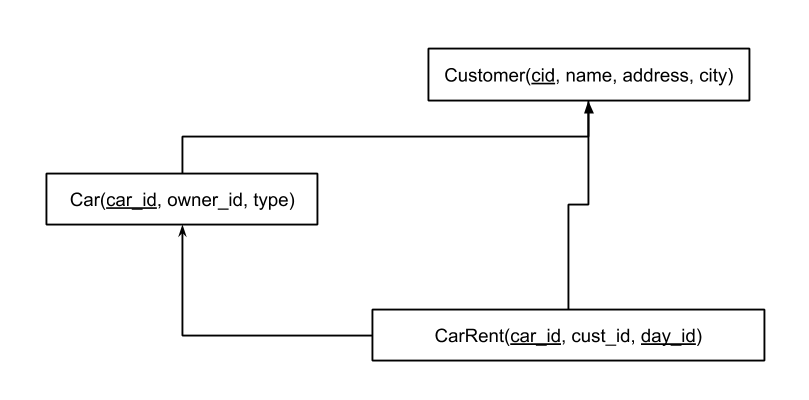
\includegraphics[width=0.6\textwidth]{LSINF2172.png}
\end{figure}

\subsection{Q1 (1pt)}
SQL to relational algebra, multiple choice question.

\subsection{Q2 (1pt)}
SQL to relational algebra.

The query counted, for each pair of city, the number of distinct days where a reservation was made by a customer of the first city, for a car owned by a customer of the second city.

\subsection{Q3 (1pt)}
Relational algebra to SQL.

\subsection{Q4 (3pt)}
ER Chen diagram of the database.

\subsection{Q5 (1pt)}
Explain a relation algebra query.

The query returned the owners that have at least two vehicles of the same type.

\subsection{Q6 (2pt)}
Given the following query in relational algebra:
\[ \pi_{type} \left( \sigma_{car_id=car_id' \wedge city="LLN"} \left( \rho_{car_id \rightarrow car_id'}(\mathrm{Car}) \bowtie \mathrm{Customer} \bowtie \mathrm{CarRent} \right) \right). \]

Optimise it as much as possible. It is not mandatory to use the procedure given during the lectures.

\subsection{Q7 (2pt)}
Find all index of a SQL query. Note that the database is likely to contain thousands of records for each city and for each day.

The query was something like "Count the number of rides (per type of vehicle?) where the day\_id > 55 and the city is Bastogne".

\nosolution

\section{Part II - Multiple choices questions (9pt)}

\subsection{Q8 (1pt)}
Find which statements were correct in a relational algebra with NULL values. The three statements included an outer join between R1(A, B) and R2(B, C) with diverse combinations of selection upon A or B, first on R1 and R2, or on (R1 outer join R2).

\subsection{Q9 (1pt)}
Find relational algebra query with not empty result

The table was
\begin{center}
\begin{tabular}{|c|c|}
    \hline
    a1 & b1 \\
    \hline
    a1 & b2 \\
    \hline
    a2 & b1 \\
    \hline
\end{tabular}
\end{center}

Some of the queries were
\begin{itemize}
    \item $\{t.A | R(t) \wedge t.A = "a1"\}$ (true)
    \item $\{t.A | R(t) \wedge \forall t' (R(t') \implies t'.A = "a1")\}$ (true)
    \item $\{t.A | R(t) \wedge \forall t' (t'.A = "a1" \implies R(t'))\}$ (true)
    \item One more that was probably false
\end{itemize}

\subsection{Q10 (1pt)}
FD equivalence
A -> B C D E
C -> D E
C, D -> E
D, E -> C

\subsection{Q11 (1pt)}
FD, find if NF1, NF2, NF3, BCNF.

The table contained

\begin{center}
\begin{tabular}{|c|c|c|c|}
    \hline
    A & B & C & D \\
    \hline
    a1 & b1 & c1 & d1 \\
    \hline
    a1 & b2 & c2 & d2 \\
    \hline
    a2 & b1 & c2 & d3 \\
    \hline
    a2 & b2 & c2 & d2 \\
    \hline
\end{tabular} 
\end{center}

\subsection{Q12 (1pt)}
Lecture 7: Questions 5.

\subsection{Q13 (1pt)}
Question about transaction, lecture 9 question 6.

\subsection{Q14 (1pt)}
Question about finding the good database system.

\subsection{Q15 (1pt)}
Overview Questions (1) Q13.

\subsection{Q16 (1pt)}
About neo4J.

\nosolution

\end{document}
